\documentclass[a4paper]{article}

% -----------------------------------Packages--------------------------------- %

% Allow to use é, é, ç, … directly from keyboard
\usepackage[utf8]{inputenc}

% T1 font encoding is an 8-bit encoding and uses fonts that have 256 glyphs
% (e.g. 'ö' is a single glyph and is not made by adding accent to 'o')
\usepackage[T1]{fontenc}

% Set the language of the document (e.g. title, section, abstract, …)
\usepackage[english]{babel}

% math stuff: equation, declaring operators, …
\usepackage{amsmath}

% math additional symbols: mathbb (blackboard font), mathfrak (Fraktur letters)
% include asmfont as a dependencies
\usepackage{amssymb}

% additional features on theorems such as theoremstyle
\usepackage{amsthm}

% bold font with \bm command
\usepackage{bm}

% enumerate lists
\usepackage{enumitem}

% import subfiles .tex
\usepackage{subfiles}

% make \ref clickale
\usepackage[hidelinks]{hyperref}

% insert appendix
\usepackage[toc,page]{appendix}

% biblatex dependency
\usepackage{csquotes}

% References loader with \addbibresource{*.bib}
\usepackage{biblatex}

% bra-ket notation
\usepackage{physics}

% add images (university logo)
\usepackage{graphicx}

% ------------------------------Bibliography---------------------------------- %

\addbibresource{references.bib}


% ------------------------------Theorems config------------------------------- %

\theoremstyle{definition}
\newtheorem{definition}{Definition}[section]
\newtheorem{theorem}{Theorem}[section]
\numberwithin{equation}{section}


% ------------------------------Customs commands------------------------------ %

% Custom command
\newcommand{\field}[1]{\mathbb{#1}}       % Complex, Real, Natural, …
\DeclareMathOperator{\Lagr}{\mathcal{L}}  % Lagrangian
\DeclareMathOperator{\U}{\mathcal{U}}     % Unitary operator


% ----------------------------------Layout------------------------------------ %

\setlength{\parindent}{0pt}


% ----------------------------------Document---------------------------------- %

\title{Higher-Order Lagrangians in classical and quantum systems}
\author{Simone Bertolotto\\[1.0em]{\small Supervisor: Prof.\ Igor Pesando}}


\begin{document}

  \begin{titlepage}
  \newcommand{\HRule}{\rule{\linewidth}{0.5mm}}

  \center
  \textsc{\textbf{\LARGE Università degli Studi di Torino}}\\[0.5cm]
  \textsc{\textbf{\Large Dipartimento di Fisica }}\\[1cm]


  \HRule\\[0.4cm]
  {\Large\bfseries Higher-Order Lagrangians in classical and quantum systems}
  \\[0.1cm] % Title of your document
  \HRule\\[0.4cm]

  \vfill
  \begin{figure}[h]
  \centering
  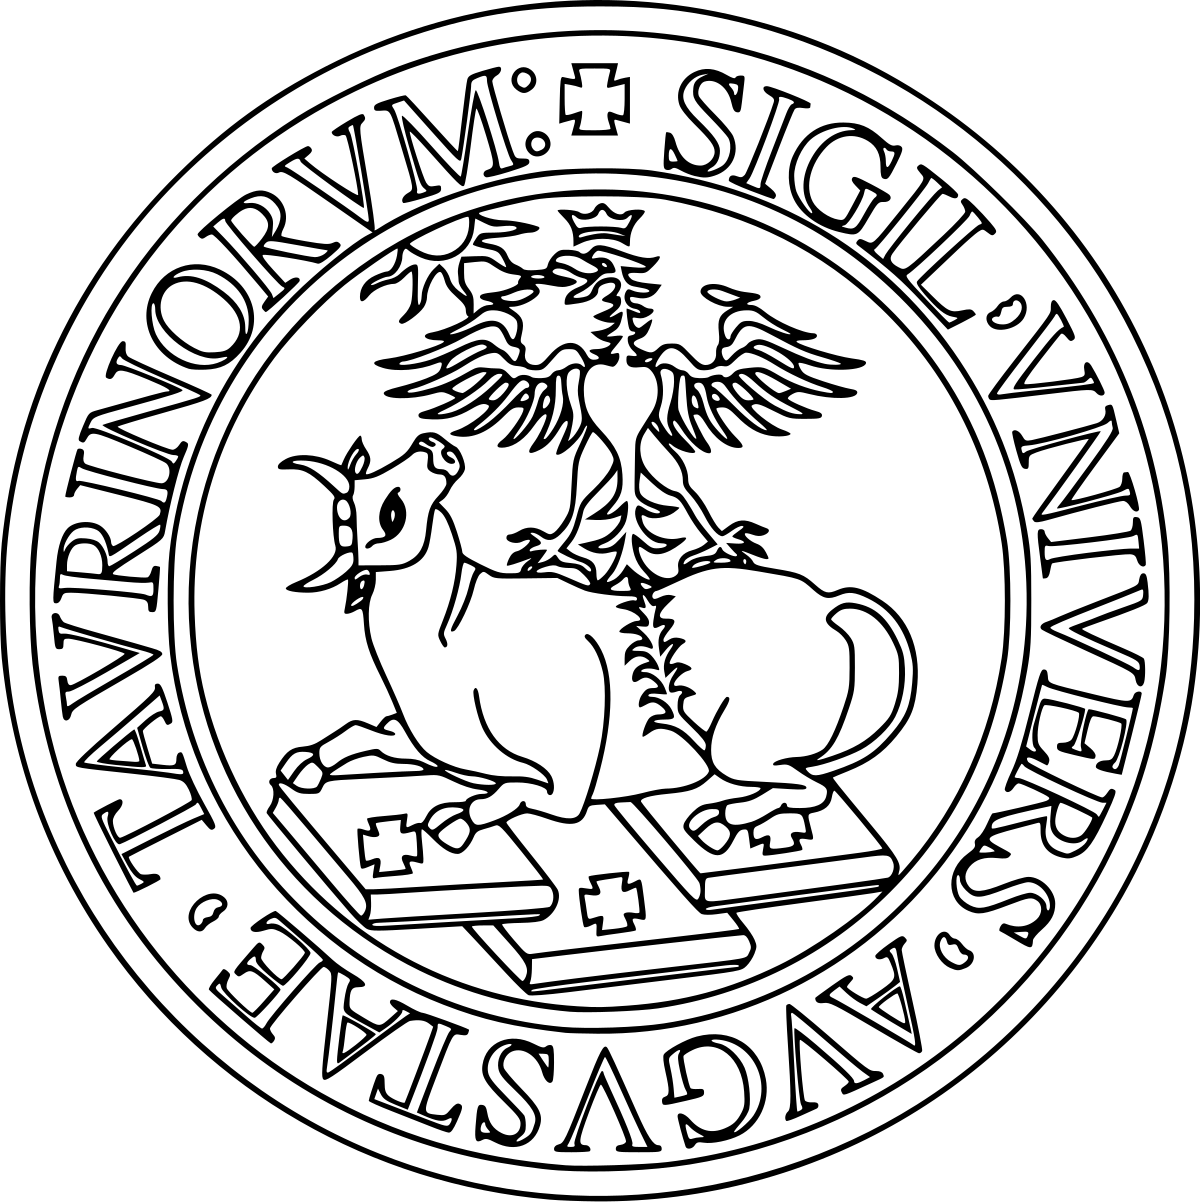
\includegraphics[scale=0.15]{logo.png}
  \end{figure}
  \vfill

  \begin{figure}[h]
  \centering
  \begin{minipage}{0.4\textwidth}

  \Large
  \textbf{\textit{Author}\\
    Simone\\ \textsc{Bertolotto}} % Author's name

  \end{minipage}
  \qquad \qquad \qquad
  \begin{minipage}{0.4\textwidth}

  \begin{flushright}
  \Large
  \textbf{\textit{Supervisor}\\
    Prof.\ Igor\\ \textsc{Pesando}} % Supervisor's name
  \end{flushright}

  \end{minipage}
  \end{figure}

  \vfill
  \textbf{{\Large December 2020}}

  \end{titlepage}

  \tableofcontents

  \newpage

  \begin{abstract}
    Usually Lagrangians depends on $q$ and $\dot{q}$ but higher order Lagrangian
    can emerge in some situations. One such situation is describe in the
    Introduction. Then a brief review of Lagrangian and Hamiltonian formalism
    is given which are used to expose the core problem of higher order
    theories (Ostrogradskian instability). One way to cure Ostrogradskian
    instability is presented in Section~\ref{section: classical higher
    derivative systems}. Finally the quantum counter part of the
    previous classical systems are explore.
  \end{abstract}\vspace{5em}

  % \newpage

  \section{Introduction}\label{section: introduction}
  \subfile{introduction}

  \section{Lagrangian and Hamiltonian formalism}\label{section: lagrangin and
  hamiltonian formalism}
  \subfile{lagrangian-and-hamiltonian-formalism}

  \section{Classical higher derivative systems}\label{section: classical higher
  derivative systems}
  \subfile{classical-higher-derivative-systems}

  \section{Quantum higher derivative systems}\label{section: quantum higher
  derivative systems}
  \subfile{quantum-higher-derivative-systems}

  \newpage

  \section{Summary}\label{section: summary}
  \subfile{summary}

  \newpage

  \begin{appendices}
    \section{Calculus of variations}\label{appendix: calculus of variation}
    \subfile{calculus-of-variations}

    \section{Canonical quantization}\label{appendix:canonical_quantization}
    \subfile{canonical-quantization}
  \end{appendices}

  \newpage

  \printbibliography{}

\end{document}
